\documentclass[journal]{IEEEtran}

\usepackage{circuitikz}   
\usepackage{tikz}
\usepackage[spanish, es-noshorthands]{babel}
\usepackage{float}
\usepackage{instructivo}
\usepackage{tabularx}
\usepackage{array}
\newcolumntype{Y}{>{\raggedright\arraybackslash}X}
\graphicspath{{./}{./fig/}}
\usepackage[natbib=true,style=trad-unsrt,backend=biber]{biblatex}
\addbibresource{literatura.bib}

\hyphenation{op-tical net-works semi-conduc-tor}

\usepackage{amsmath}
\usetikzlibrary{shapes, arrows.meta, positioning, calc}
 
% --- Estilos ---
\tikzset{
  block/.style={
    draw, rectangle,
    minimum width=3.2cm, minimum height=1.2cm,
    align=center, font=\small
  },
  line/.style={draw, -{Latex[length=2.5mm, width=2mm]}},
  siglabel/.style={font=\footnotesize, text=blue!65!black},
  blklabel/.style={font=\footnotesize, right=0.15cm, text=black}
}

\begin{document}
\setlength{\parindent}{4.2mm}
\title{Planta térmica TCLab}

\author{Matías~A.~Camacho,~\IEEEmembership{Estudiante,~TEC}
        y~Juan~P.~Elizondo,~\IEEEmembership{Estudiante,~TEC}
}

% The paper headers
\markboth{Laboratorio de control automático, IIS2026}%
{Laboratorio de control automático}


% make the title area
\maketitle


%%%%%%%%%%%%%%%%%%%%%%%%%%%%%%%%%%%%%%%%%%%%%%%%%%%%%%%%%%%%%%%%%%%%%%%%%%%%%%%%%%%%%%%%%%%%%%
%%%%%%%%%%%%%%%%%%%%%%%%%%%%%%%%%%%%%%%%%%%%%%%%%%%%%%%%%%%%%%%%%%%%%%%%%%%%%%%%%%%%%%%%%%%%%%
\section{Introducción}

\IEEEPARstart{E}{l} desarrollo de sistemas de control modernos para aplicaciones industriales y electrónicas 
requiere metodologías que garanticen la precisión, seguridad y robustez del diseño antes de su despliegue 
físico. En este contexto, el Diseño Basado en Modelos (\textit{Model-Based Design}) ofrece un marco estructurado 
que utiliza modelos matemáticos ejecutables para representar tanto la planta física como los algoritmos de 
control. Dentro de este ciclo de desarrollo, la prueba \textit{Model-in-the-Loop} (MIL) constituye la primera etapa de 
verificación funcional, permitiendo simular y analizar el comportamiento del lazo cerrado en un entorno 
puramente virtual.

En esta práctica de laboratorio se aborda la caracterización, identificación y control de temperatura de la planta 
física \textit{Temperature Control Lab} (TCLab). La dinámica térmica del sistema se analiza inicialmente a partir de primeros 
principios mediante un balance de energía no lineal que contempla pérdidas por convección y radiación. Dado que las 
técnicas de control lineal convencionales se basan en representaciones en el dominio de Laplace, el modelo no lineal 
se aproxima mediante linealización analítica e identificación experimental.
%%%%%%%%%%%%%%%%%%%%%%%%%%%%%%%%%%%%%%%%%%%%%%%%%%%%%%%%%%%%%%%%%%%%%%%%%%%%%%%%%%%%%%%%%%%%%%
%%%%%%%%%%%%%%%%%%%%%%%%%%%%%%%%%%%%%%%%%%%%%%%%%%%%%%%%%%%%%%%%%%%%%%%%%%%%%%%%%%%%%%%%%%%%%%
\section{Modelado e Identificación del Sistema}
\subsection{Modelo físico}
En la guía de laboratorio proporcionada \cite{guia_tclab_2026}, se desarrolló el modelo físico de la planta a partir de principios termodinámicos, 
con los cuales resultó un modelo no lineal que posteriormente se linealizó al rededor de $Q = 50\%$.
Tras el proceso de linealización, se logra llegar a la siguiente función de transferencia, correspondiente a la planta de
análisis:

\begin{equation}
        \begin{aligned}
                G(s) &= \frac{K}{\tau s + 1} \\
                \tau &= -\frac{1}{\gamma} \\
                K    &= \frac{1}{\gamma} \\
        \end{aligned}
\end{equation}

La planta utilizada en este laboratorio cuenta con dos calentadores resistivos ($Q_1$ y $Q_2$), así como dos sensores
de temperatura ($T_1$ y $T_2$) según se muestra en la Figura \ref{fig:planta}. De las partes anteriores, se utilizan 
únicamente el primer calentador, así como la temperatura medida por $T_1$.

De esta forma, al energizar $Q_1$, una parte de la energía eléctrica se convierte en calor, llegando a elevar la
temperatura del conjunto calentador-sensor.

\begin{figure}[H]
        \centering
        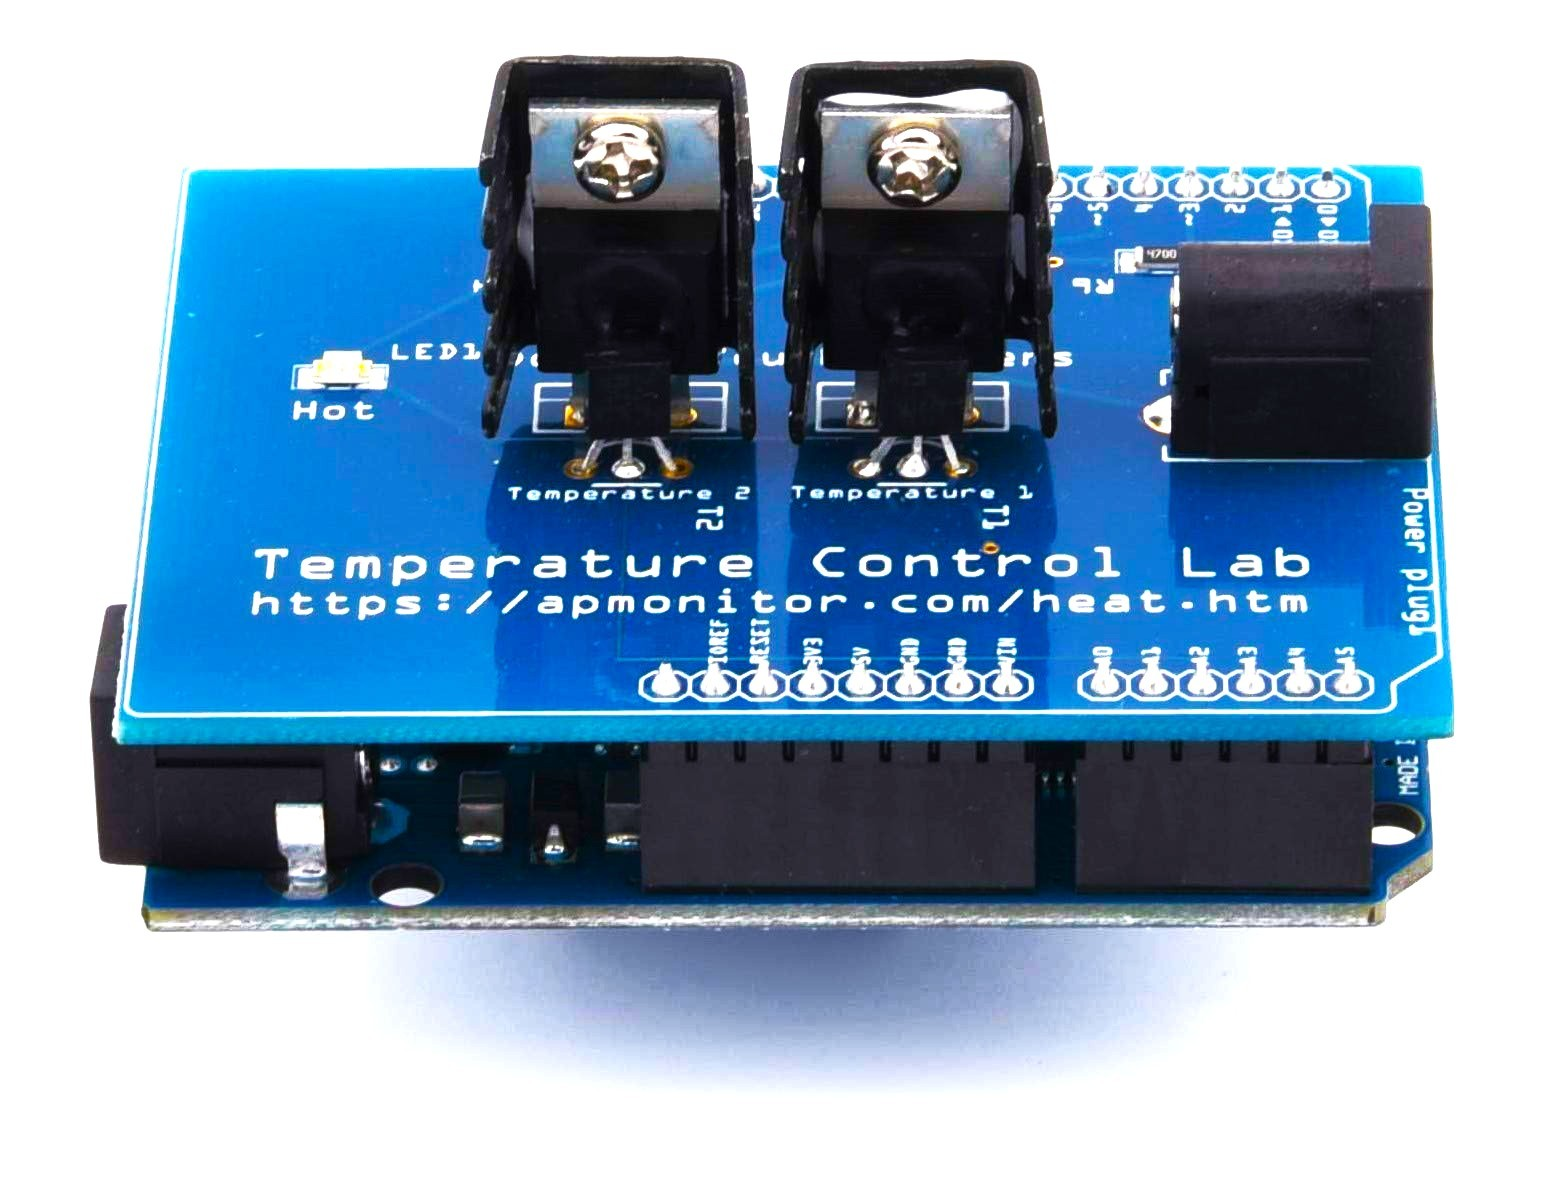
\includegraphics[width=0.65\linewidth]{TCLab.jpg}
        \caption{Planta TCLab}
        \label{fig:planta}
\end{figure}

Durante el proceso de identificación de modelos \textit{First-Order Plus Dead Time} (FOPDT), con el fin de representar la dinámica térmica dominante de 
la TCLab, se utiliza un modelo de primer orden y con tiempo muerto, para la función de transferencia de la
planta, tal como se muestra en la ecuación \ref{eq:G_fopdt}.

\begin{equation}
        \begin{aligned}
                G_p{(s)} &= \frac{K }{\tau s + 1} \cdot e^{-\theta s} \\
        \end{aligned}
\label{eq:G_fopdt}
\end{equation}

En la siguiente tabla, se resume un registro inicial de la planta a tratar. Así como de las condiciones del entorno
que resultan relevantes para la ejecución de este laboratorio. 

\begin{table}[H]
  \centering
  \caption{Registro inicial de la planta y el entorno}
  \label{tab:registro_planta}
  \renewcommand{\arraystretch}{1.5}
  \begin{tabularx}{\columnwidth}{@{}lX@{}}
    \toprule
    \textbf{Dato} & \textbf{Valor registrado} \\
    \midrule
    Código de la TCLab           & -- \\
    Fecha y hora                 & 12/08/2026 - 7:40~a.m. \\
    Integrantes                  & Matías~A.~Camacho~y~Juan~P.~Elizondo\\
    Puerto de comunicación       & /dev/ttyS0 (Linux) \\
    Temperatura ambiente inicial & $24.51~^\circ\mathrm{C}$ \\
    Observaciones del montaje    & N/A \\
    \bottomrule
  \end{tabularx}
\end{table}

\subsection{Identificación experimental}


\subsection{Validación y selección del modelo}


%%%%%%%%%%%%%%%%%%%%%%%%%%%%%%%%%%%%%%%%%%%%%%%%%%%%%%%%%%%%%%%%%%%%%%%%%%%%%%%%%%%%
%%%%%%%%%%%%%%%%%%%%%%%%%%%%%%%%%%%%%%%%%%%%%%%%%%%%%%%%%%%%%%%%%%%%%%%%%%%%%%%%%%%%
\section{Diseño del controlador y evaluación MIL}
\subsection{Diseño del controlador PI}

\subsection{Evaluación Model-in-the-Loop (MIL)}


%%%%%%%%%%%%%%%%%%%%%%%%%%%%%%%%%%%%%%%%%%%%%%%%%%%%%%%%%%%%%%%%%%%%%%%%%%%%%%%%%%%%
%%%%%%%%%%%%%%%%%%%%%%%%%%%%%%%%%%%%%%%%%%%%%%%%%%%%%%%%%%%%%%%%%%%%%%%%%%%%%%%%%%%%
\section{Generación de código y verificación de software}
\subsection{Implementación del controlador}
\subsection{Inspección del código generado}
\subsection{Verificación Software-in-the-loop (SIL)}

%%%%%%%%%%%%%%%%%%%%%%%%%%%%%%%%%%%%%%%%%%%%%%%%%%%%%%%%%%%%%%%%%%%%%%%%%%%%%%%%%%%%
%%%%%%%%%%%%%%%%%%%%%%%%%%%%%%%%%%%%%%%%%%%%%%%%%%%%%%%%%%%%%%%%%%%%%%%%%%%%%%%%%%%%
\section{Verificación Processor-in-the-loop (PIL)}



%%%%%%%%%%%%%%%%%%%%%%%%%%%%%%%%%%%%%%%%%%%%%%%%%%%%%%%%%%%%%%%%%%%%%%%%%%%%%%%%%%%%
%%%%%%%%%%%%%%%%%%%%%%%%%%%%%%%%%%%%%%%%%%%%%%%%%%%%%%%%%%%%%%%%%%%%%%%%%%%%%%%%%%%%
\section{Implementación experimental}


%%%%%%%%%%%%%%%%%%%%%%%%%%%%%%%%%%%%%%%%%%%%%%%%%%%%%%%%%%%%%%%%%%%%%%%%%%%%%%%%%%%%
%%%%%%%%%%%%%%%%%%%%%%%%%%%%%%%%%%%%%%%%%%%%%%%%%%%%%%%%%%%%%%%%%%%%%%%%%%%%%%%%%%%%
\section{Discusión}

%%%%%%%%%%%%%%%%%%%%%%%%%%%%%%%%%%%%%%%%%%%%%%%%%%%%%%%%%%%%%%%%%%%%%%%%%%%%%%%%%%%%
%%%%%%%%%%%%%%%%%%%%%%%%%%%%%%%%%%%%%%%%%%%%%%%%%%%%%%%%%%%%%%%%%%%%%%%%%%%%%%%%%%%%
\section{Conclusiones}

%%%%%%%%%%%%%%%%%%%%%%%%%%%%%%%%%%%%%%%%%%%%%%%%%%%%%%%%%%%%%%%%%%%%%%%%%%%%%%%%%%%%
%%%%%%%%%%%%%%%%%%%%%%%%%%%%%%%%%%%%%%%%%%%%%%%%%%%%%%%%%%%%%%%%%%%%%%%%%%%%%%%%%%%%


\printbibliography

%%%%%%%%%%%%%%%%%%%%%%%%%%%%%%%%%%%%%%%%%%%%%%%%%%%%%%%%%%%%%%%%%%%%%%%%%%%%%%%%%%%%
%%%%%%%%%%%%%%%%%%%%%%%%%%%%%%%%%%%%%%%%%%%%%%%%%%%%%%%%%%%%%%%%%%%%%%%%%%%%%%%%%%%%
\section{Biografías de los autores}

 
\begin{IEEEbiographynophoto}{Matías A. Camacho}
        Estudiante del Instituto Tecnológico de Costa Rica (TEC) en la carrera de ingeniería electrónica.
        
        Correo: jeacamacho@estudiantec.cr
\end{IEEEbiographynophoto}

\begin{IEEEbiographynophoto}{Juan P. Elizondo}
        Estudiante de Ingeniería Electrónica en el Tecnológico de Costa Rica (TEC).
        Cuenta con preparación y/o experiencia en áreas como:
        \begin{itemize}
            \item Arquitectura básica de redes, CISCO CCNA V7 (ITN), (2021).
            \item Fundamentos de ciberseguridad, CISCO Systems, (2022).
            \item Programa de tutorías estudiantiles, Tecnológico de Costa Rica, (2024).
            \item Diseño de circuitos digitales, TEC (2025).
        \end{itemize}
        
        Correo: juelizondo@estudiantec.cr
\end{IEEEbiographynophoto}


\vfill

\end{document}